\documentclass[12pt,aspectratio=169]{beamer}


\usepackage{algorithm,algorithmic}

\usepackage[utf8]{inputenc}
\usepackage{booktabs}
\usepackage[opacity=0.1]{pdfcomment} % set to 0 to make annotation icons invisible
\usepackage{pdfpc}
\usepackage{arev}
\usepackage{multicol}

\usepackage{xcolor, color, colortbl}
\definecolor{dkgreen}{rgb}{0,0.5,0}
\definecolor{dkred}{rgb}{0.8,0,0}
\definecolor{dkblue}{rgb}{0,0,0.5}
\definecolor{gray}{rgb}{0.5,0.5,0.5}
\definecolor{mauve}{rgb}{0.58,0,0.82}
\definecolor{hilight}{RGB}{122,86,0}

\definecolor{LRed}{rgb}{1,.8,.8}
\definecolor{MRed}{rgb}{1,.6,.6}
\definecolor{HRed}{rgb}{1,.2,.2}

\usepackage{tikz}
\usetikzlibrary{arrows.meta,
                calc, chains,
                quotes,
                positioning,
                shapes.geometric}


\def\scalefact{0.85}
\newcommand{\cev}[1]{\reflectbox{\ensuremath{\vec{\reflectbox{\ensuremath{#1}}}}}}
\newcommand{\evalat}[2]{\left.#1\right\vert_{#2}}

\newcommand{\znode}[5][black]{\path (#3,#4) node(#2) [circle,draw,color=#1] {#5};}
\newcommand{\zunedge}[6][black]{%
\begin{scope}
	\path (#2,#3) node(this) [inner sep=0pt,triangle,draw,color=#1] {#4};
	\draw[->,color=#1] (#5) -- (this.west);
	\draw[->,color=#1] (this.east) -- (#6);
\end{scope}}
\newcommand{\zbiedge}[7][black]{%
\begin{scope}
	\path (#2,#3) node(this) [inner sep=0pt,triangle,draw,color=#1] {#4};
	\draw[->,color=#1] (#5) -- (this);
	\draw[->,color=#1] (#6) -- (this);
	\draw[->,color=#1] (this.east) -- (#7);
\end{scope}}
\newcommand{\zedge}[5][black]{\path (#3,#4) node(#2) [inner sep=0pt,triangle,draw,color=#1] {#5};}

\definecolor{blue(pigment)}{rgb}{0.2, 0.2, 0.6}
\definecolor{burgundy}{rgb}{0.5, 0.0, 0.13}


\usepackage{listings}
%% \usetheme{Goettingen}
\usefonttheme{serif}
\usepackage{times}
\setbeamertemplate{navigation symbols}{}

\title{Deep Learning}
\subtitle{Lecture 5: Multilayer Perceptrons}
 
 
%\author[Mehrdad Maleki] % (optional, for multiple authors)
%{Mehrdad Maleki, Barak A. Pearlmutter\footnote{ Institute & Department of Computer Science
%Maynooth University, Co. Kildare, Ireland}, Jeffrey Mark Siskind}
 
%\institute[NUIM] % (optional)
%{
%  Department of Computer Science \\
%  National University of Ireland Maynooth
 
%}

\author[]{\textbf{Dr. Mehrdad Maleki}}
%\institute[]{\textsuperscript{1}Department of Computer Science\\ National University of Ireland\\ Maynooth}
% 
\date{}
 
%\logo{\includegraphics[height=1.5cm]{lion-logo.png}}

\renewcommand{\Re}{\mathbb{R}}
 
\begin{document}
 
\frame{\titlepage}

\begin{frame}
We have seen that $x_1+x_2\geq 2$ is the half-plane that recognize $x_1\wedge x_2$ and this graph shows why,
\begin{center}
\begin{tikzpicture}[fill opacity=0.5]
\draw[->] (0,0) -- (0,3);
\draw[->] (0,0) -- (3,0);

\node[right] at (3,0) {$x_1$};
\node[left] at (0,3) {$x_2$};
\pause
\fill[green] (0,1) circle (2pt);
\fill[green] (1,0) circle (2pt);
\fill[green] (0,0) circle (2pt);
\fill[red] (1,1) circle (2pt);
\pause
\node[left] at (0,0) {$(0,0)$};
\node[below] at (1,0) {$(1,0)$};
\node[left] at (0,1) {$(0,1)$};
\node[right] at (1,1) {$(1,1)$};
\pause
\draw[pink] (2,0) -- (0,2);
\pause
\draw[fill=pink,draw=none, rotate around={(45:(2,0)}] (2,0) rectangle (4,2.8);
\end{tikzpicture}
\end{center}
\end{frame}

\begin{frame}
We have seen that we can't compute XOR with a single perceptron.
\begin{center}
\begin{tikzpicture}[fill opacity=0.5]
\draw[->] (0,0) -- (0,3);
\draw[->] (0,0) -- (3,0);

\node[right] at (3,0) {$x_1$};
\node[left] at (0,3) {$x_2$};
\pause
\fill[red] (0,1) circle (2pt);
\fill[red] (1,0) circle (2pt);
\fill[green] (0,0) circle (2pt);
\fill[green] (1,1) circle (2pt);
\pause
\node[left] at (0,0) {$(0,0)$};
\node[below] at (1,0) {$(1,0)$};
\node[left] at (0,1) {$(0,1)$};
\node[right] at (1,1) {$(1,1)$};
\pause
\draw[pink] (0.5,0) -- (0,0.5);
\draw[pink] (1.6,0) -- (0,1.6);
\pause
\draw[fill=pink,draw=none, rotate around={(45:(0.5,0)}] (0.5,-1) rectangle (1.3,2.8);
\end{tikzpicture}
\end{center}
\end{frame}


\begin{frame}
\begin{itemize}
\item But with two perceptrons we can compute XOR, because,
\bigskip
\item $x\oplus y=(\overline{x}\wedge y)\vee (x\wedge \overline{y})$.
\end{itemize}

\end{frame}

\begin{frame}
\begin{center}
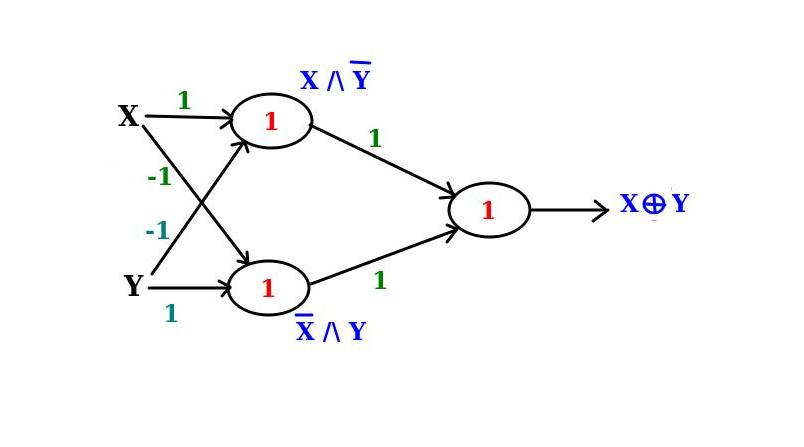
\includegraphics[scale=0.6]{nonlinear_xor}
\end{center}
\end{frame}

\begin{frame}
\frametitle{Depth of a Graph}
The length of the longest path in Directed Acyclic Graph (DAG) from the source to the sink is the \textcolor{blue}{\em depth} of the graph.
\end{frame}

\begin{frame}
\begin{center}
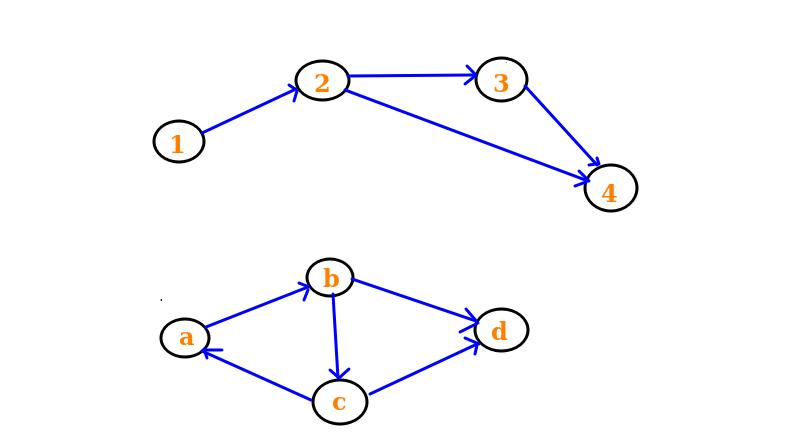
\includegraphics[scale=0.6]{depth}
\end{center}
\end{frame}

\begin{frame}
\frametitle{Feedforward Neural Network}
A \textcolor{blue}{\em Feedforward Neural Network} is a DAG of perceptrons. The depth of this DAG is the depth of the graph.
\end{frame}

\begin{frame}
\frametitle{Deep Neural Network}
A \textcolor{blue}{\em Deep Neural Network} is a feedforward neural network of the depth at least 3.
\end{frame}

\begin{frame}
\begin{center}
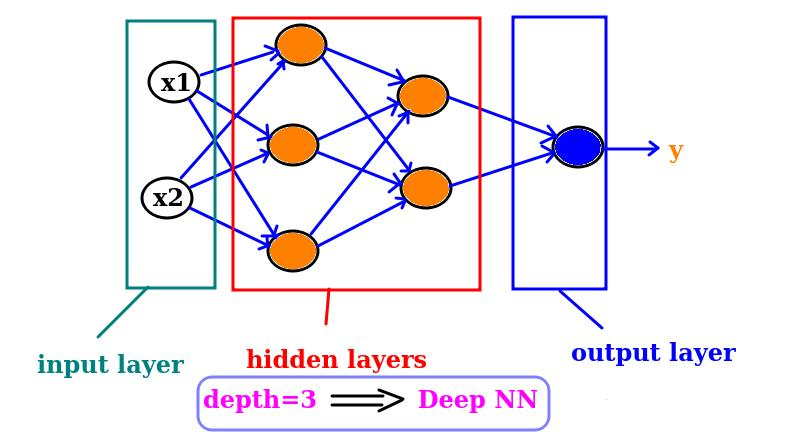
\includegraphics[scale=0.6]{deep}
\end{center}
\end{frame}

\begin{frame}
\frametitle{Universal Boolean Functions}
Multi layer perceptrons can compute any Boolean function. We say multi layer perceptrons are \textcolor{blue}{\em universal Boolean functions}. Any Boolean function can be computed by a multi layer perceptron with just one hidden layer.
\end{frame}

\begin{frame}
With the truth table of a Boolean function we can obtain a multi layer perceptrons with just one layer as follow. Write the DNF (Disjunctive Normal Form- OR of AND clauses) of the truth table and build a single perceptron per each clause and then combine them with an OR gate. 
\end{frame}

\begin{frame}
\begin{table}[h!]
\centering
 \begin{tabular}{||c c c c||} 
 \hline
 $x_1$ & $x_2$ & $x_3$ & y \\ [0.5ex] 
 \hline\hline
 0 & 1 & 1 & 1 \\ 
 1 & 1 & 0 & 1 \\
 1 & 0 & 1 & 1 \\
 1 & 1 & 1 & 1 \\ [1ex] 
 \hline
 \end{tabular}
\end{table}
$y=(\overline{x_1}\wedge x_2 \wedge x_3)\vee (x_1\wedge x_2\wedge \overline{x_3})\vee (x_1\wedge\overline{x_2}\wedge x_3)\vee (x_1\wedge x_2 \wedge x_3)$
\end{frame}

\begin{frame}
\begin{center}
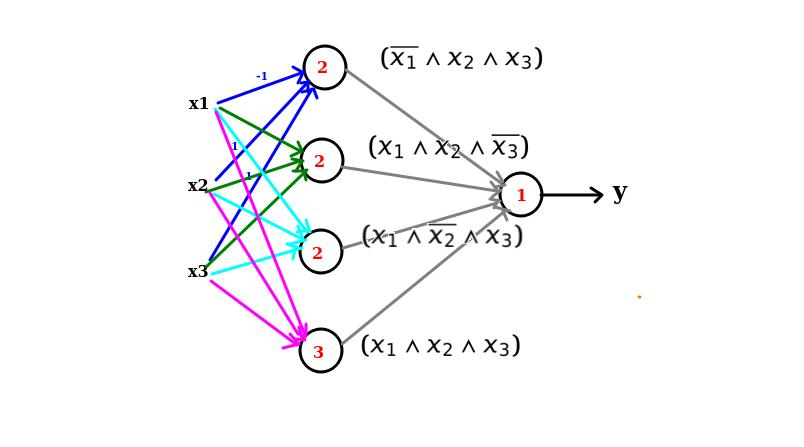
\includegraphics[scale=0.6]{dnf}
\end{center}
\end{frame}

\begin{frame}
\frametitle{Real inputs}
So far, the inputs was Boolean, i.e., $0, 1$. But the perceptrons can determine the linear classifier for the real-valued inputs. But how we can design a multi layer perceptron for decision boundary with the complex shapes?
\end{frame}



\begin{frame}
The function that inside the triangle is equal to 1 and outside of it is equal to 0.
\begin{center}
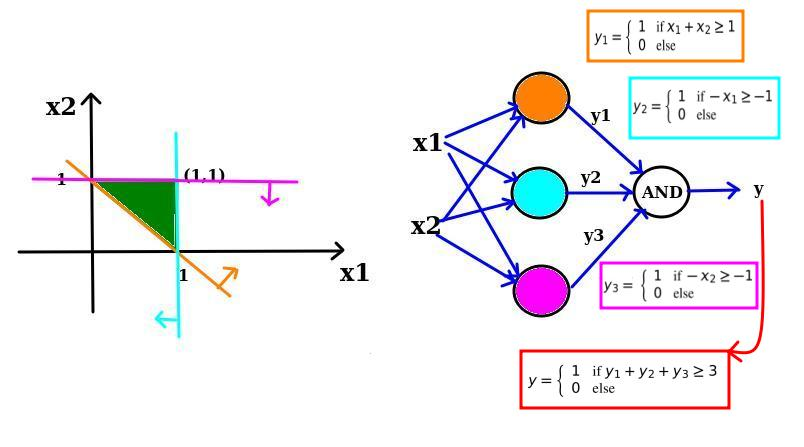
\includegraphics[scale=0.6]{triangle}
\end{center}

\end{frame}

\begin{frame}
\begin{center}
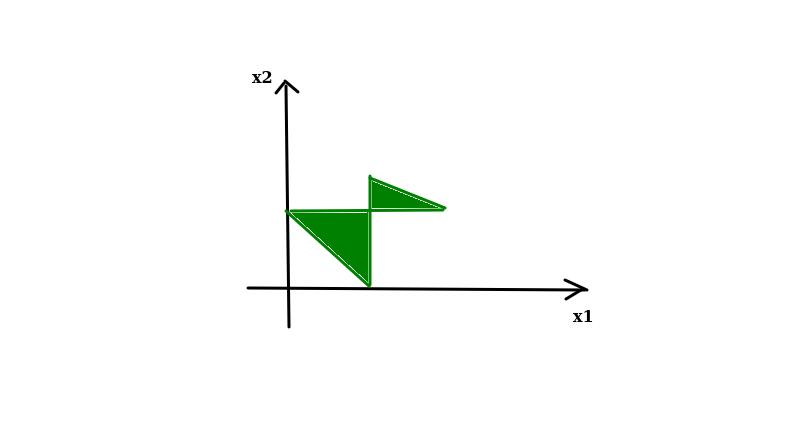
\includegraphics[scale=0.7]{two_triangle}
\end{center}
\end{frame}

\begin{frame}
\begin{center}
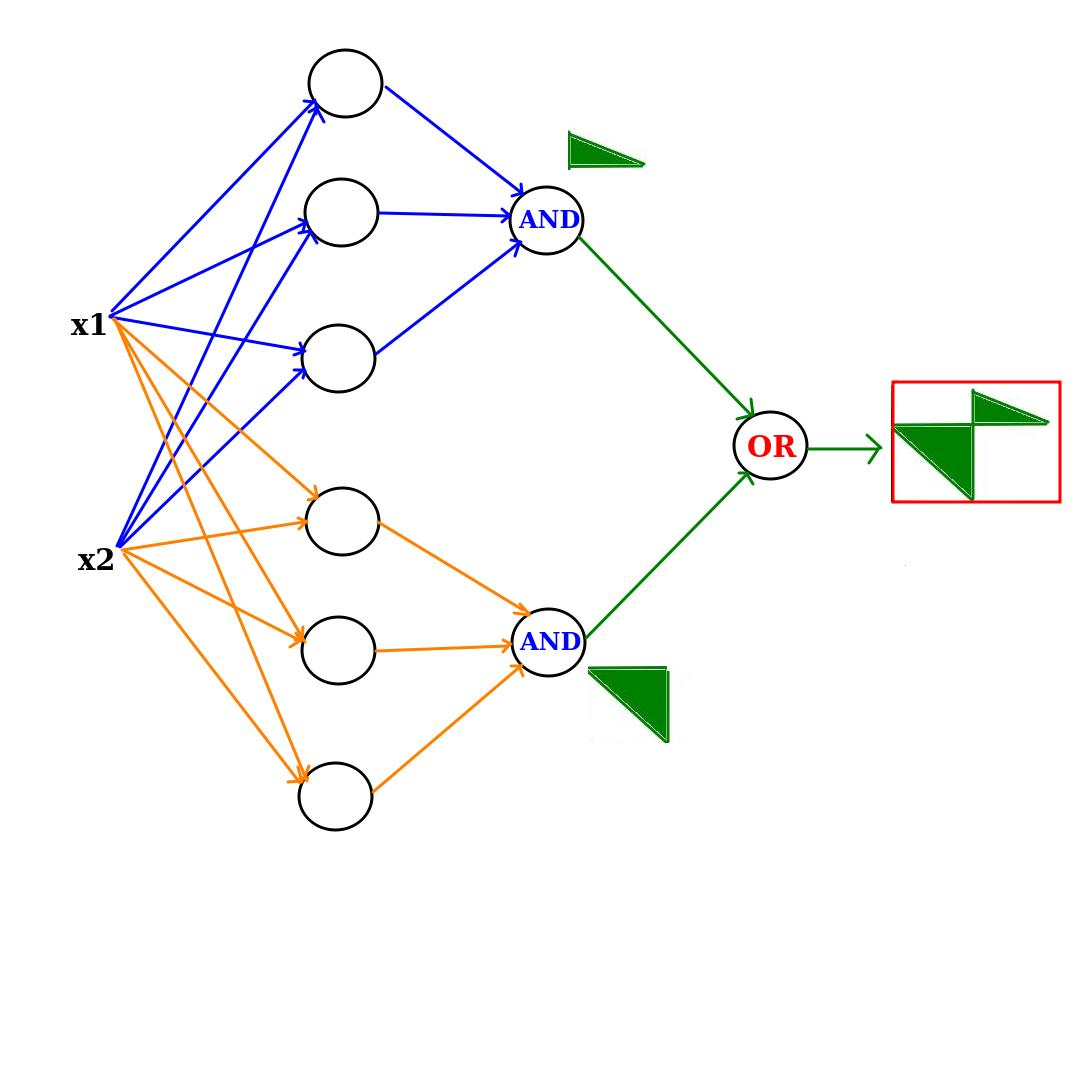
\includegraphics[scale=0.35]{two_triangle2}
\end{center}
\end{frame}


\begin{frame}
\begin{center}
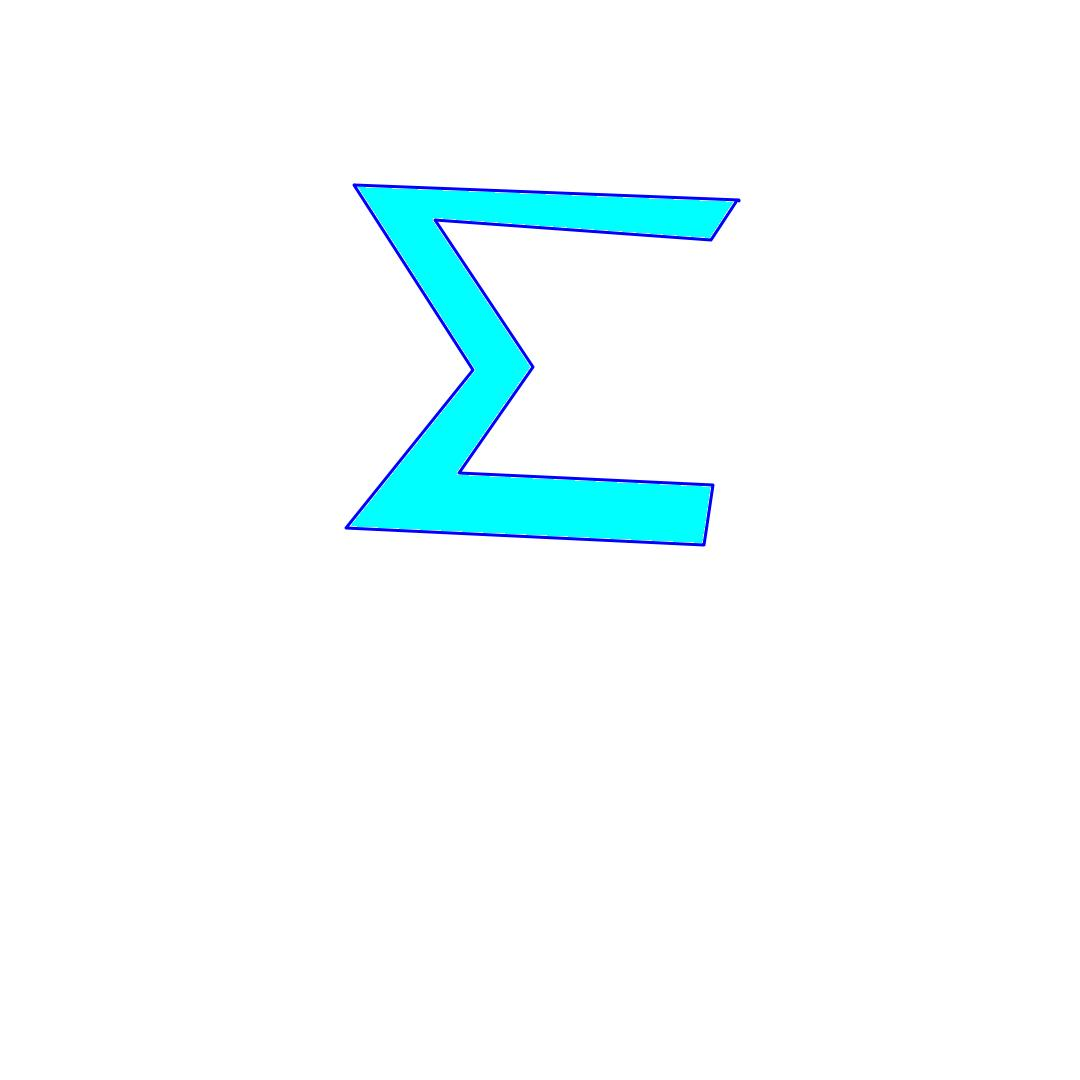
\includegraphics[scale=0.35]{sigma}
\end{center}
\end{frame}


\begin{frame}
\begin{center}
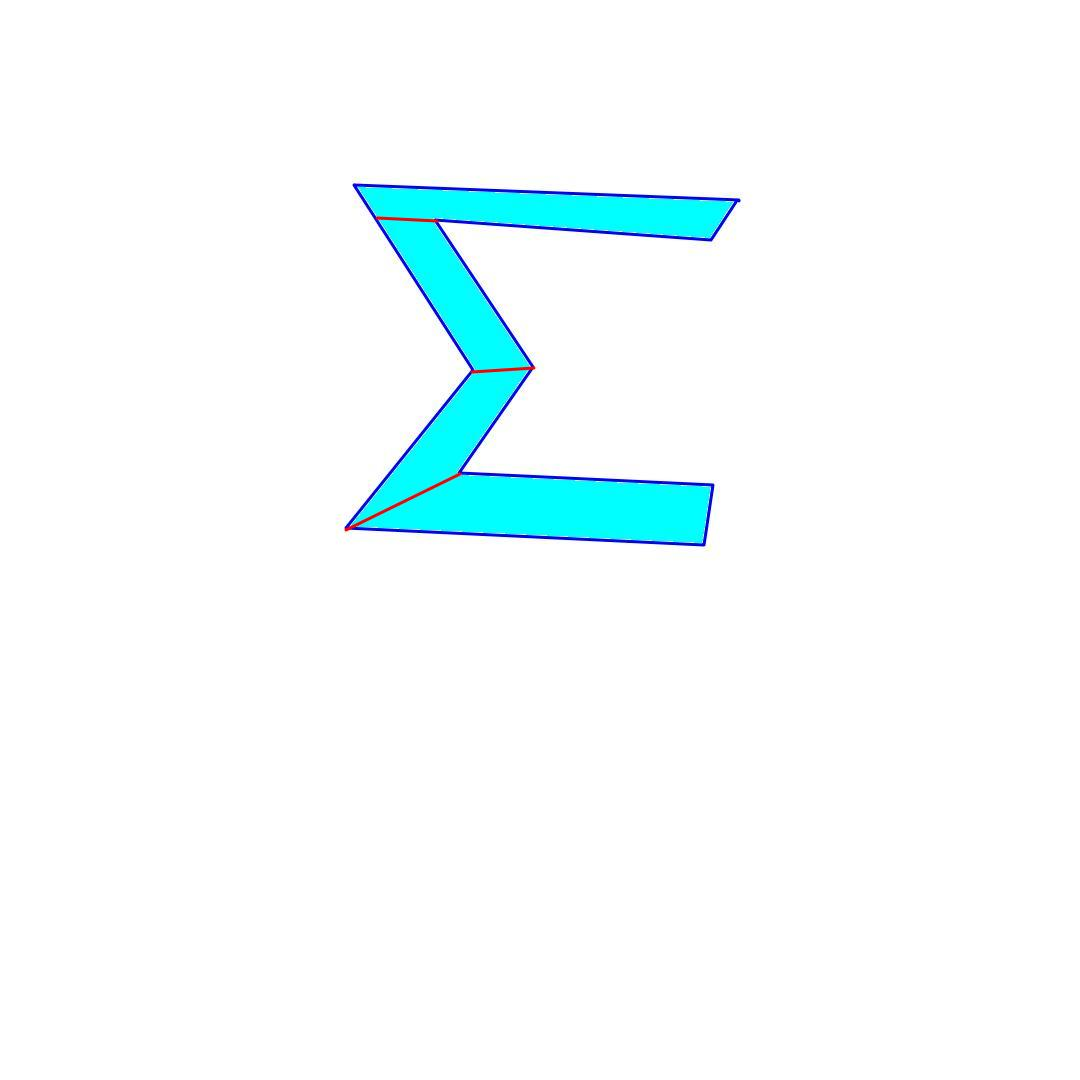
\includegraphics[scale=0.35]{sigma2}
\end{center}
\end{frame}


\begin{frame}
\begin{center}
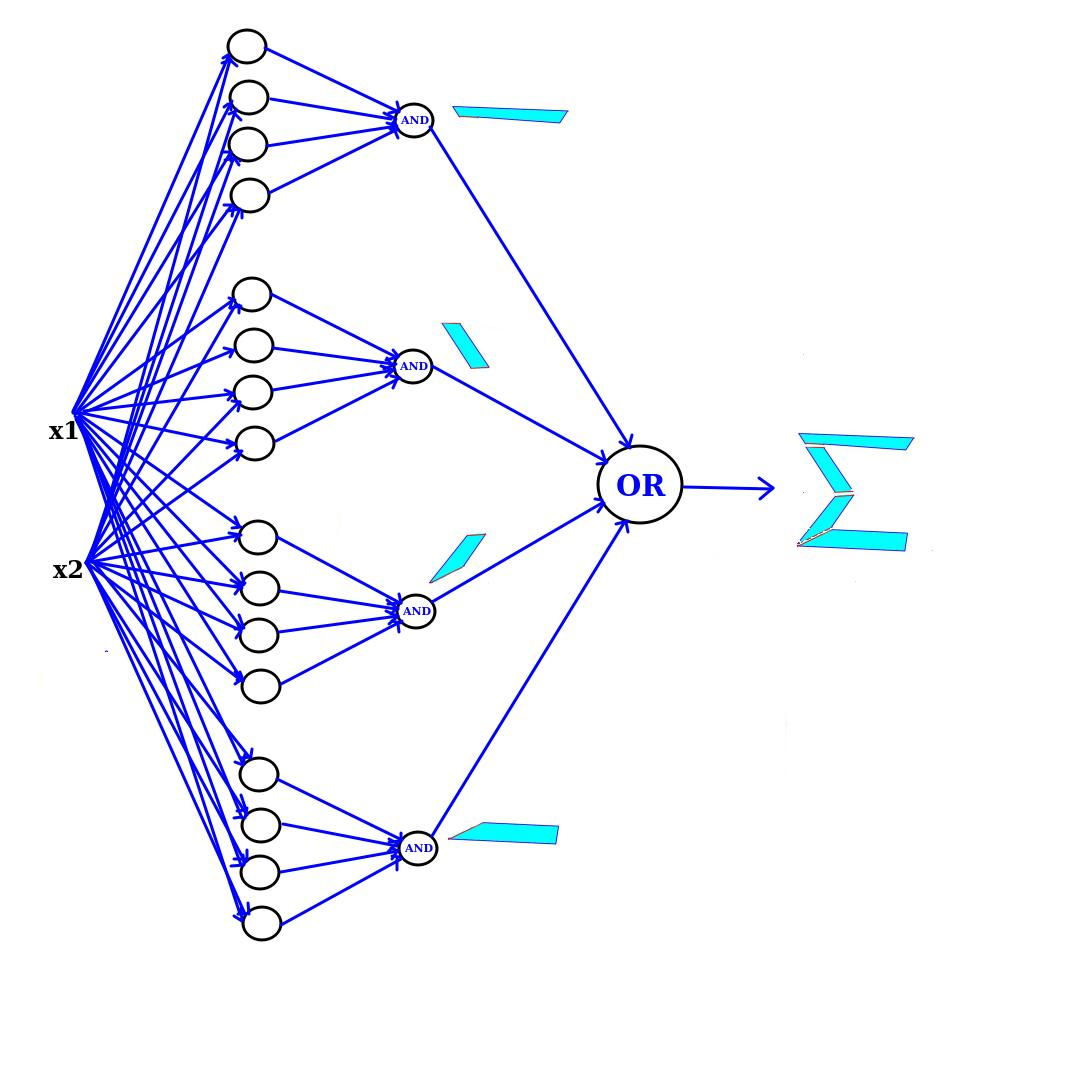
\includegraphics[scale=0.35]{sigma3}
\end{center}
\end{frame}


\begin{frame}
\begin{center}

\includegraphics[scale=0.4]{nonlinear}
\end{center}
\end{frame}


\begin{frame}
\begin{center}
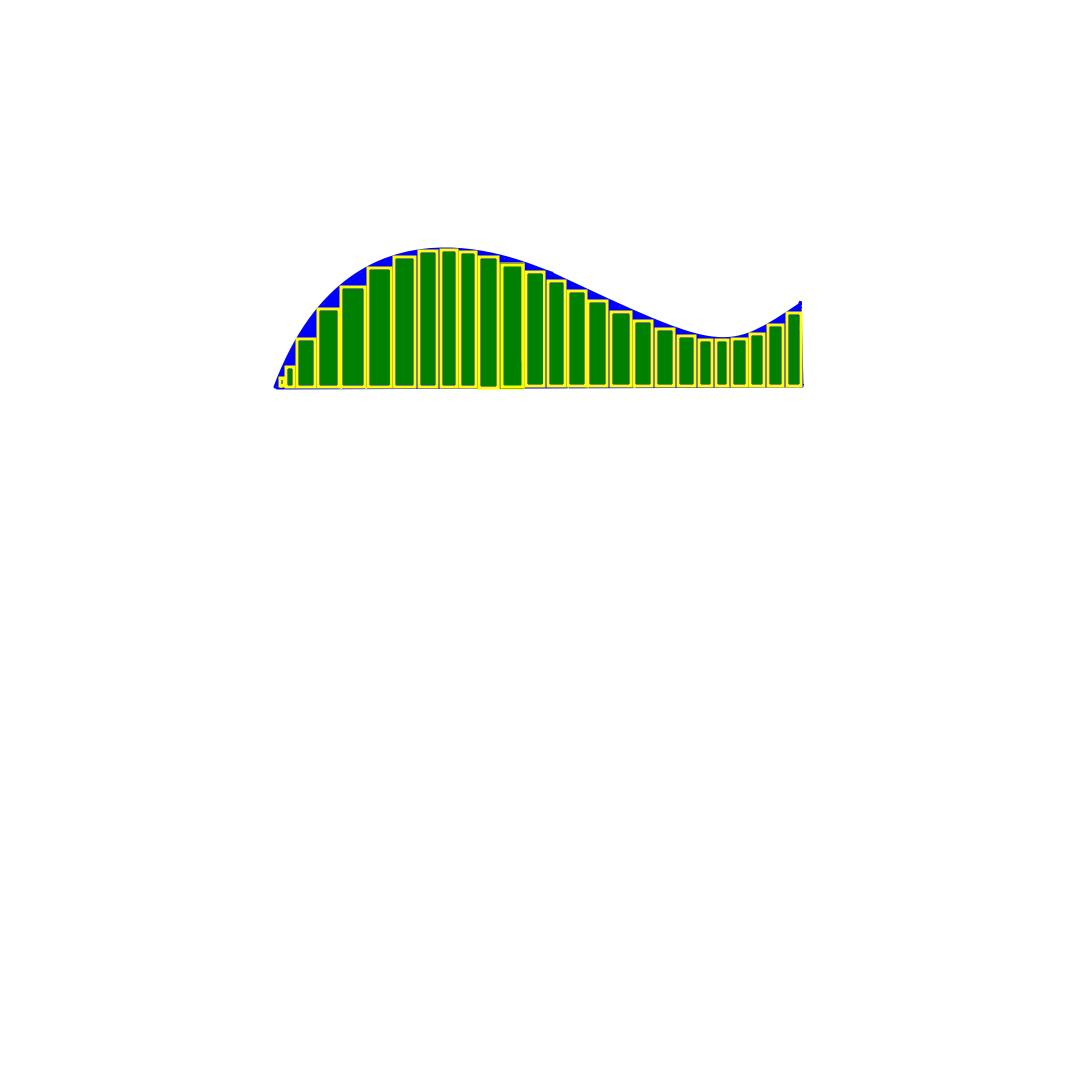
\includegraphics[scale=0.4]{nonlinear2}
\end{center}
\end{frame}


\begin{frame}
\begin{center}
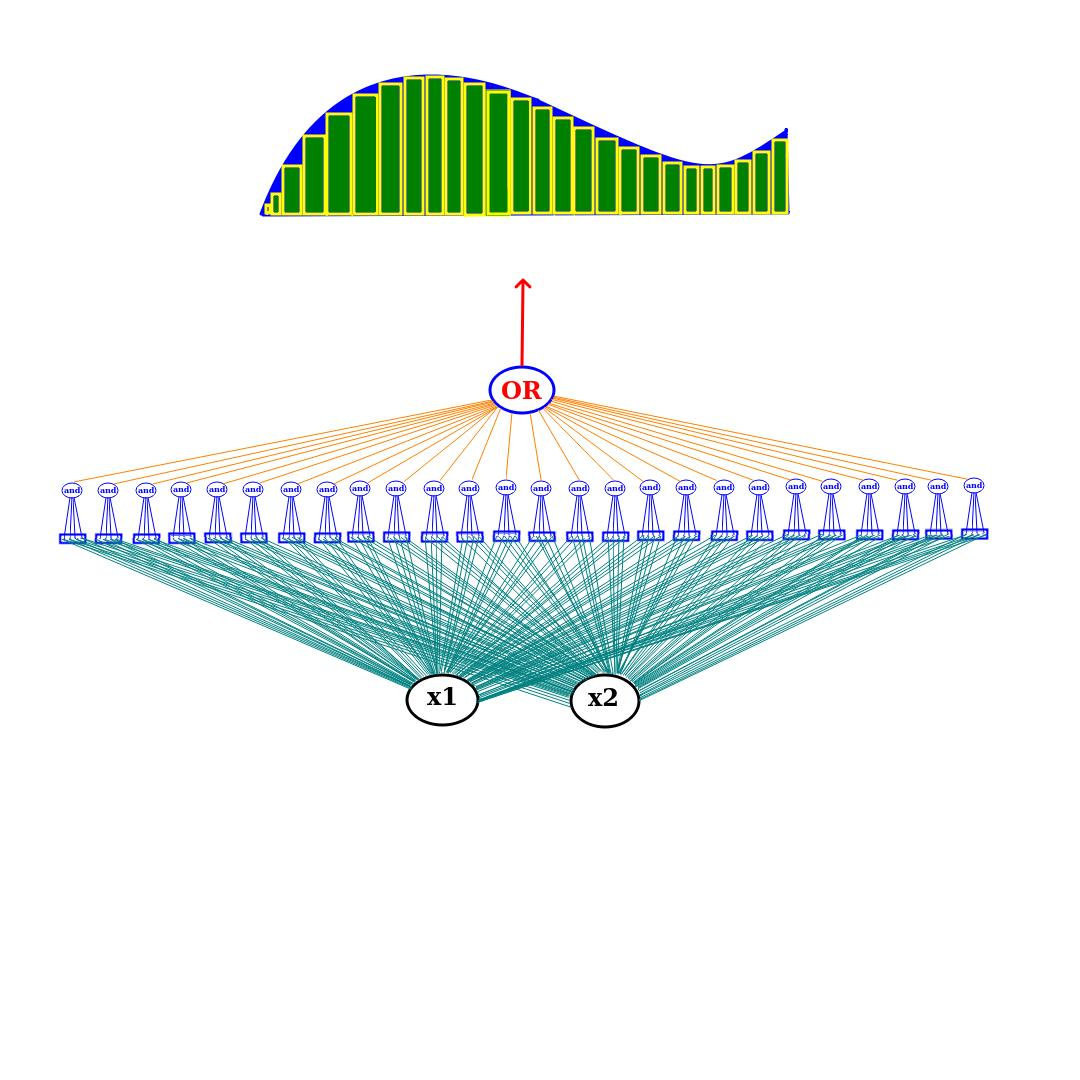
\includegraphics[scale=0.4]{nonlinear3}
\end{center}
\end{frame}


\begin{frame}
\begin{center}
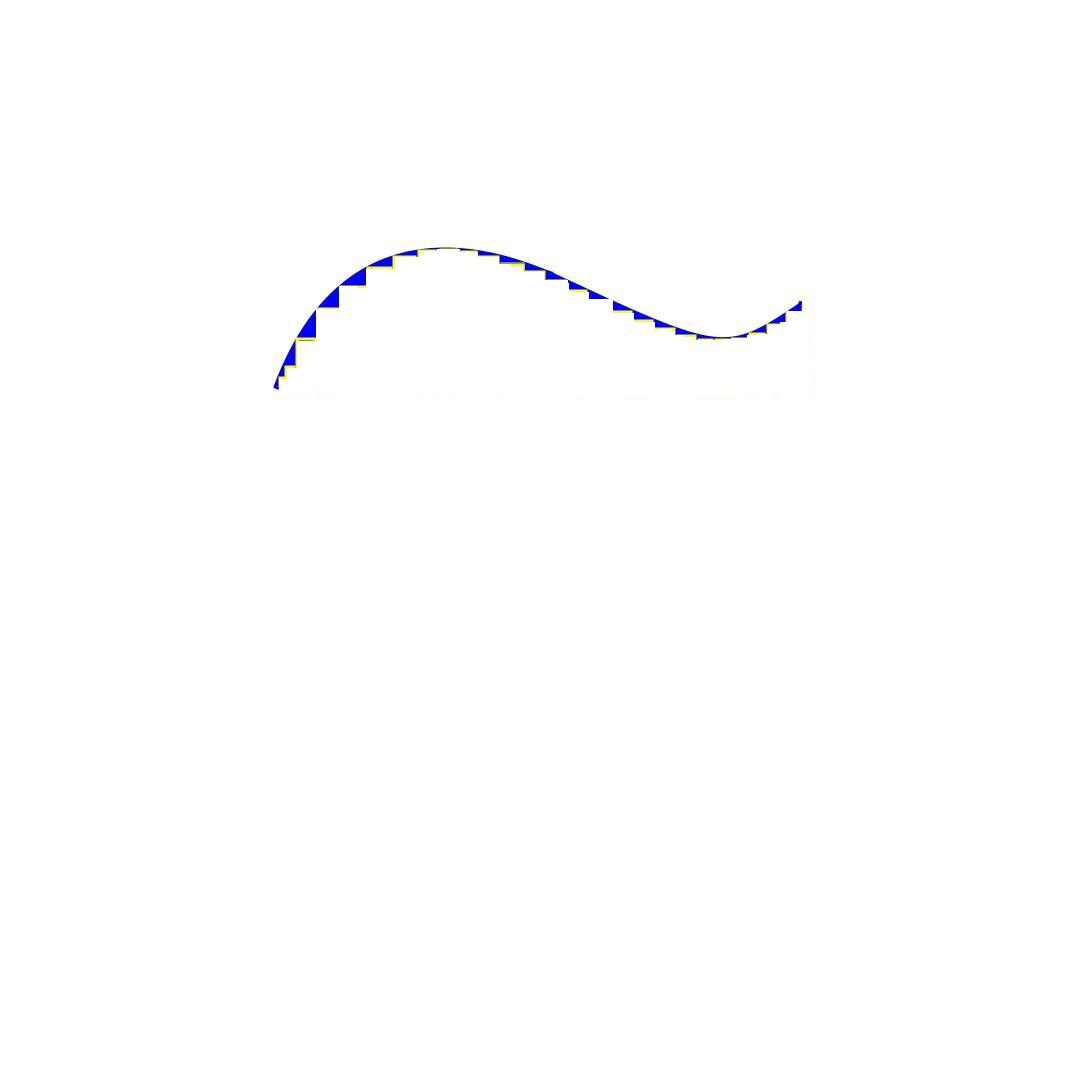
\includegraphics[scale=0.4]{nonlinear4}
\end{center}
\end{frame}


\begin{frame}
\begin{center}
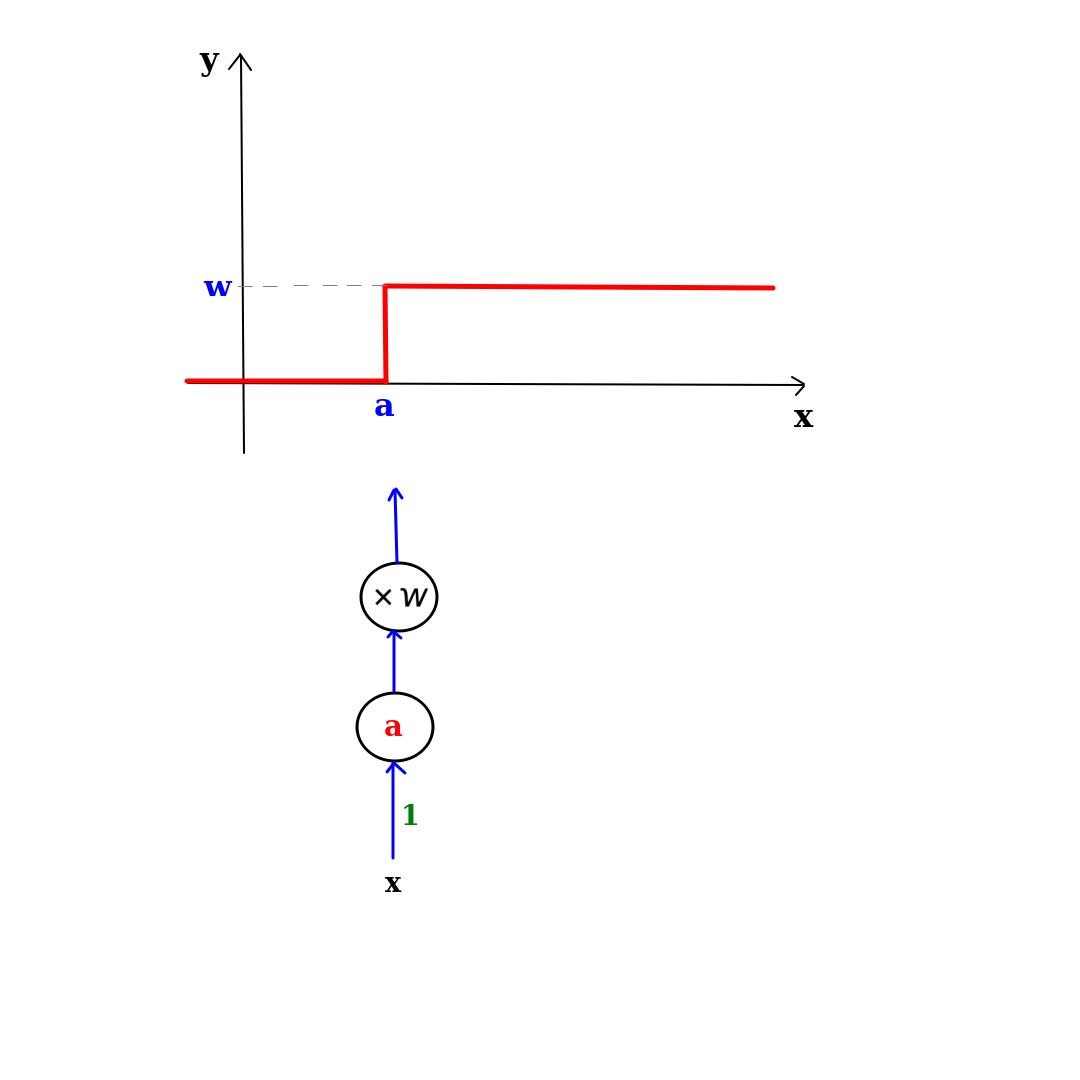
\includegraphics[scale=0.3]{step1}
\end{center}
\end{frame}


\begin{frame}
\begin{center}
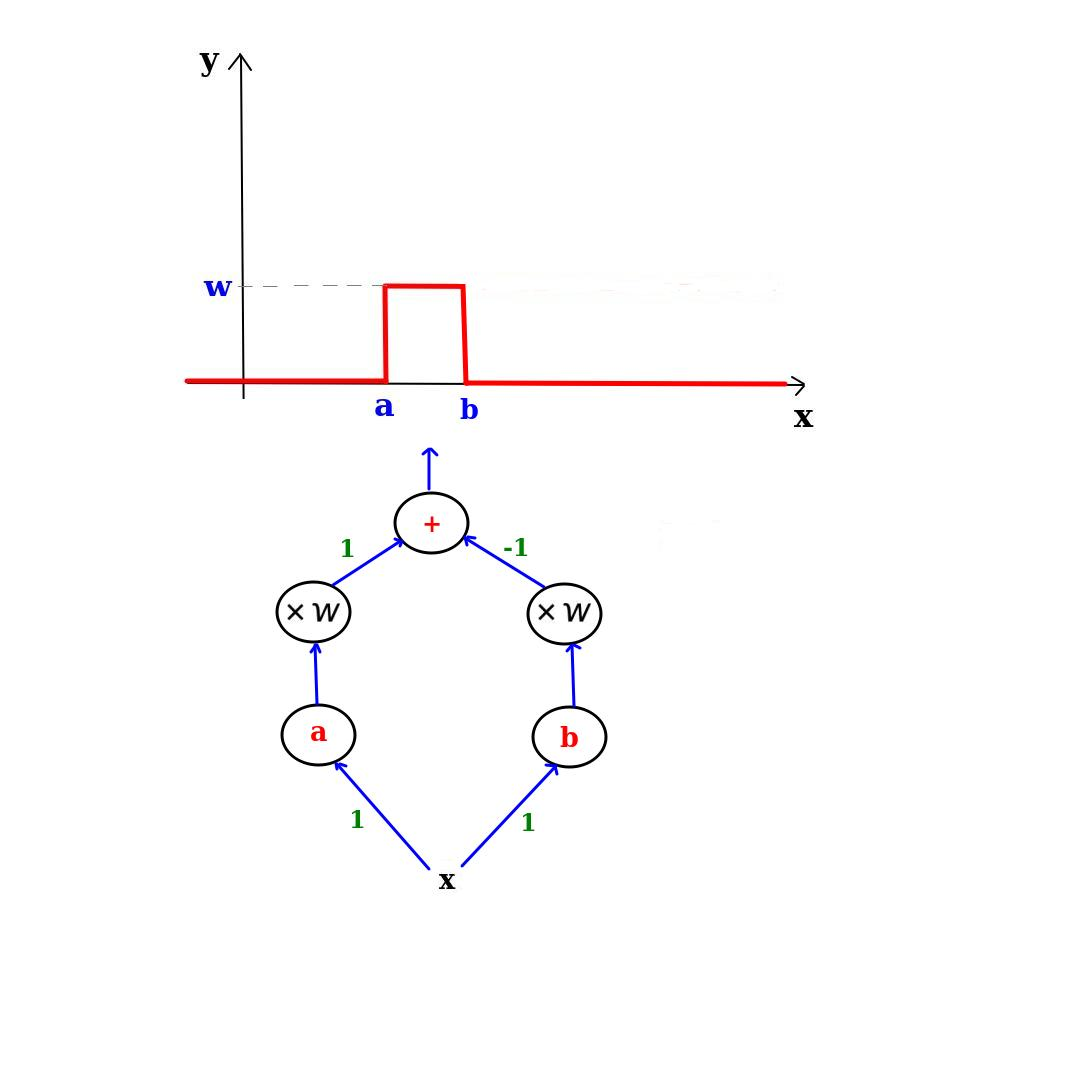
\includegraphics[scale=0.3]{step2}
\end{center}
\end{frame}


\begin{frame}
\begin{center}
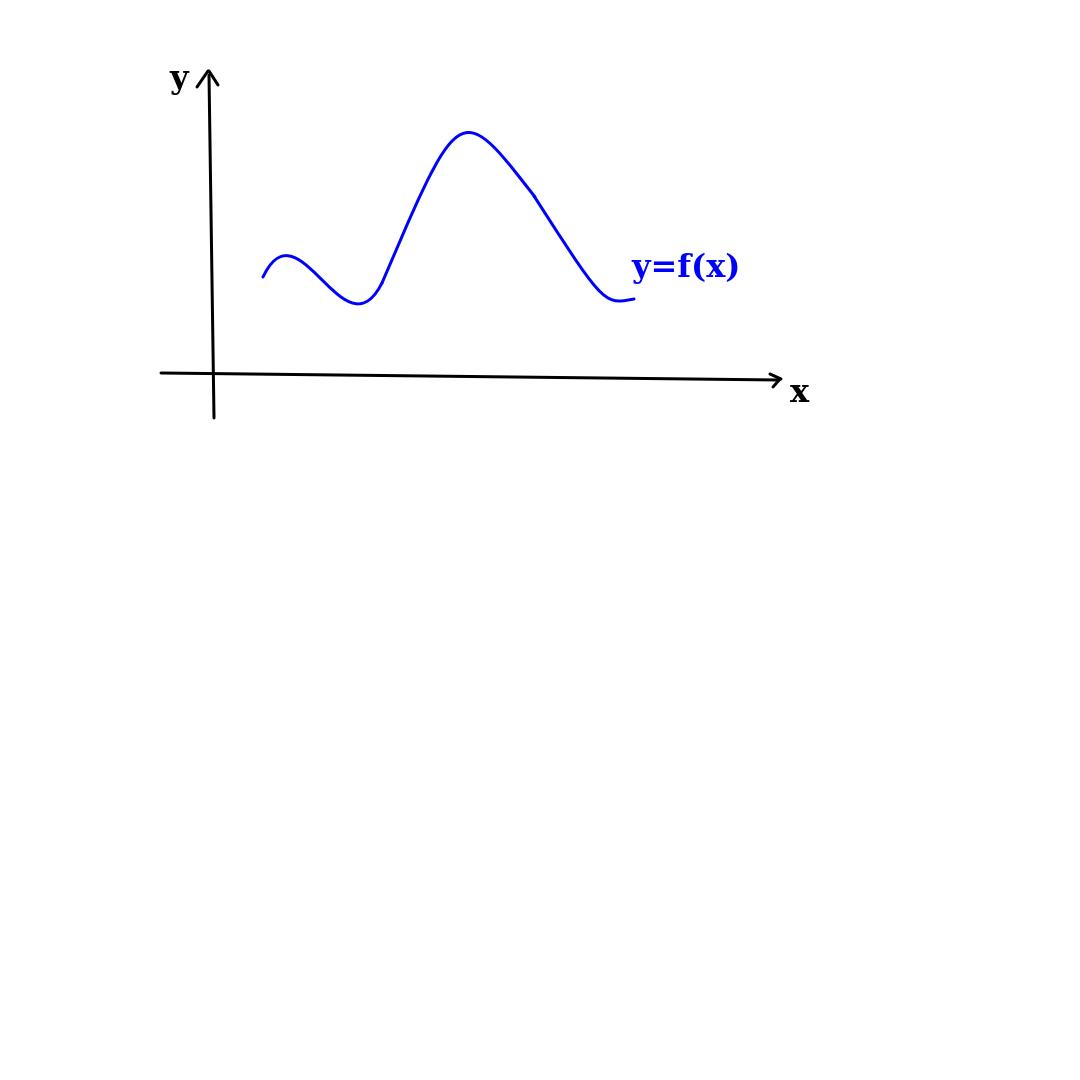
\includegraphics[scale=0.4]{real}
\end{center}
\end{frame}


\begin{frame}
\begin{center}
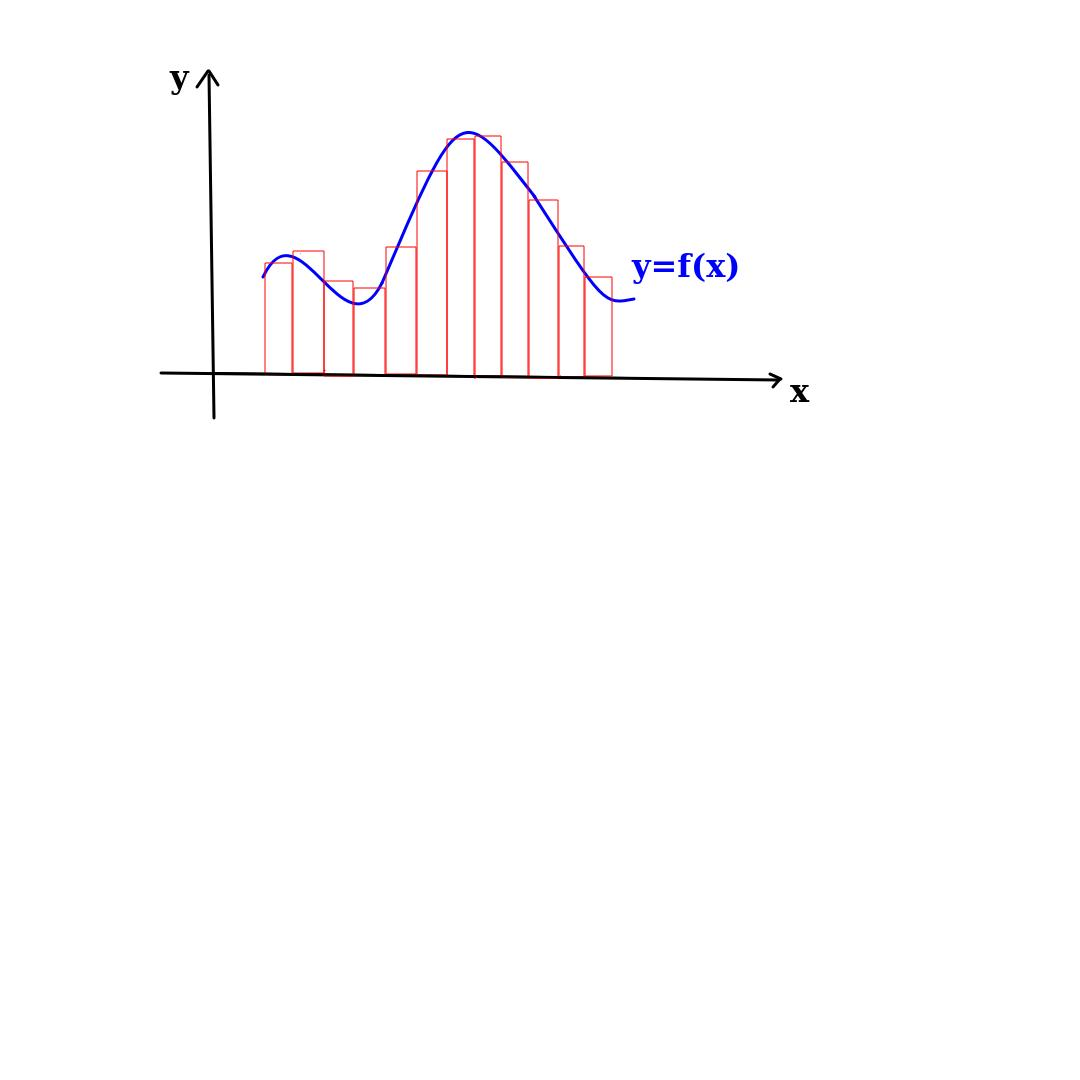
\includegraphics[scale=0.35]{real2}
\end{center}
\end{frame}


\begin{frame}
\begin{center}
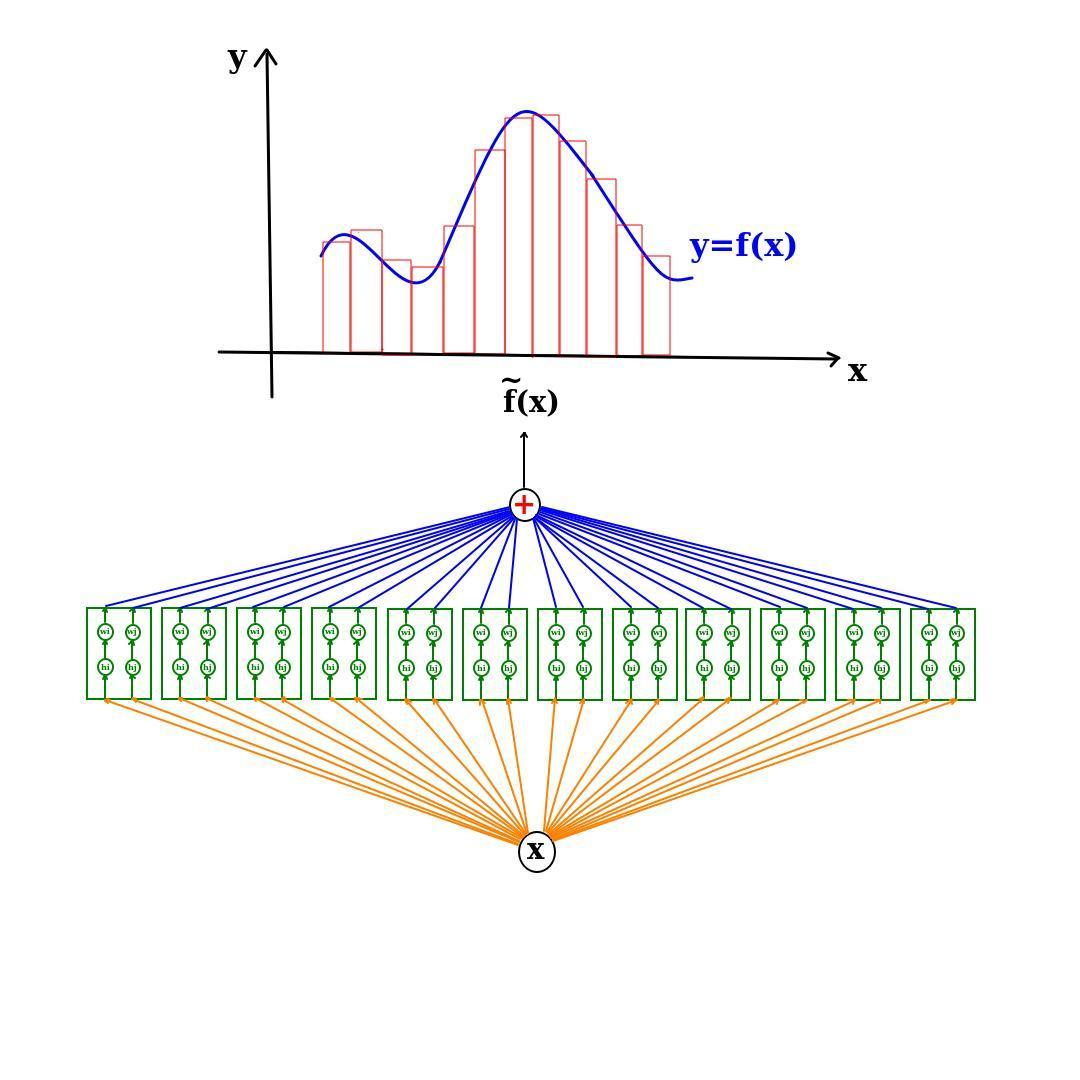
\includegraphics[scale=0.35]{real3}
\end{center}
\end{frame}

\begin{frame}
\begin{itemize}
\item Multi-layer Perceptrons are universal Boolean functions.
\bigskip
\item Multi-layer Perceptron are universal classifiers.
\bigskip
\item Multi-layer Perceptron are \textbf{universal approximators}.
\end{itemize}
\end{frame}

\begin{frame}{}
  \centering \Huge
  \emph{Thank You}
\end{frame}

\end{document}

